\chapter{Tools from Differential Geometry}\label{ch:tools}

\begin{flushright}
\emph{Give me six hours to chop down a tree\\ and I will spend the first four sharpening the axe.}
\\ -Abraham Lincoln
\end{flushright}

\vspace{0.6cm}

% % % % % % % % % % % % % % % % % % % % % % % % % % % % % % % % % % % % % %
% % % % % % % % % % % % % % % % % % % % % % % % % % % % % % % % % % % % % %
% % SECTION
% % % % % % % % % % % % % % % % % % % % % % % % % % % % % % % % % % % % % %
% % % % % % % % % % % % % % % % % % % % % % % % % % % % % % % % % % % % % %
\section{A Lie Group Structure for the Set of Transformations}\label{se:finite_lie_group}

%%introductory definition
We consider every group $\mathbb{G}$ as a group of transformations acting on $\mathbb{R}^{d}$, having in mind the particular case $d=2,3$ for 2-dimensional or 3-dimensional images.
We will focus our attention to transformations defined by matrices or diffeomorphism. Other than group they also have the structure of Lie group: they are considered with a maximal atlas that makes them differentiable manifold, in which the composition of two transformations and the inverse of each transformation are well defined differentiable maps:
\begin{align*}
\mathbb{G} \times \mathbb{G} & \longrightarrow  \mathbb{G}    \\
(x,y) &\longmapsto  x y^{-1}
\end{align*}

Differential geometry is, generally speaking, a technique to use the well known calculus features and operators on spaces different from the usual $\mathbb{R}^{n}$. Adding the differentiable structure to a group of transformations gives us new handles to hold and manipulate them: in particular provides the opportunity to define a tangent space to each point of the group (and so a fiber bundle), a space of vector fields, a set of flows and one parameter subgroup as well as other features that enrich this structure.
Due to space limitations we will refer to \cite{do1976differential} and \cite{lee2012introduction} for the definitions and concepts of differential geometry and \cite{do1992riemannian} for definition and concepts of Riemannian geometry.

% % % % % % % % % % % % % % % % % % % % % % % % % % % % % % % % % % % % % %
% % SECTION
% % % % % % % % % % % % % % % % % % % % % % % % % % % % % % % % % % % % % % 
\section{Lie Exponential, Lie logarithm, Lie log-composition and the BCH formula}\label{se:lie_exp_log_comp_bch}
Let $\mathbf{v}$ be an element in the tangent space fo the Lie group $\mathbb{G}$ indicated with $\mathfrak{g}$.
The \emph{Lie exponential} is defined as 
\begin{align*}
\exp :  \mathfrak{g} & \longrightarrow  \mathbb{G}  \\
\mathbf{v} &\longmapsto  \exp(\mathbf{v} ) = \gamma(1) %\quad \dot{\gamma}(t) = V_{\gamma(t)}, \gamma(0) = e
\end{align*}
where $\gamma: [0,1]\rightarrow \mathbb{G} $ is the unique one-parameter subgroup of $\mathbb{G}$ having $\mathbf{v}$ as its tangent vector at the identity (\cite{do1992riemannian}, \cite{ebin2006singularities}, \cite{Arsigny:MRM:06}).
It satisfies the following properties:
\begin{enumerate}
	\item $\exp(t\mathbf{v}) =\gamma(t) $.
	\item $\exp(\mathbf{v}) = e$ if $\mathbf{v} = \mathbf{0}$.
	\item $\exp(\mathbf{v})\circ \exp(\mathbf{-v})  = e$
	\item It satisfies the one parameter subgroup property:
	\begin{align*}
	\exp((t+s)\mathbf{v}) = \gamma(t+s) = \gamma(t)\circ \gamma(s) = \exp(t\mathbf{v})\exp(s\mathbf{v})
	\end{align*}
	\item $\exp(\mathbf{v})$ is invertible and $(\exp(\mathbf{v}))^{-1} = \exp(-\mathbf{v})$.
		\item  $\exp(\mathbf{u} + \mathbf{v}) =\lim_{m\rightarrow \infty} (\exp(\frac{\mathbf{v}}{m}) \circ\exp(\frac{\mathbf{v}}{m}))^{m}$
	\item $\exp$ is a local isomorphism: which means that it is an isomorphisms between a neighborhood of $\mathbf{0}$ in $\mathfrak{g}$ to a neighborhood of $e$ in $\mathbb{G}$.
\end{enumerate}
The neighborhoods of $\mathbb{G}$ and of $\mathfrak{g}$ such that the last property holds, are called \emph{internal cut locus} of $\mathbb{G}$ and $\mathfrak{g}$ respectively. The \emph{cut locus} is the boundary of the internal cut locus.

When we deal with a matrix Lie group of dimension $n$, the composition in the Lie group consists in the matrix product and we have the following remarkable properties \cite{hall2015lie}, \cite{kirillov2008introduction}:
\begin{enumerate}
	\item for all $\mathbf{v}$ in a matrix Lie algebra $\mathfrak{g}$:
	\begin{align}\label{eq:exp_as_inf_sum}
	\exp(\mathbf{v}) = \sum_{k=0}^{\infty} \frac{\mathbf{v}^{k}}{k!}
	\end{align}
	\item If $\mathbf{u}$ and $\mathbf{v}$ are commutative then $\exp(\mathbf{u} + \mathbf{v}) = \exp(\mathbf{u})\exp(\mathbf{v})$.
	\item If $\mathbf{c}$ is an invertible matrix then $\exp(\mathbf{c}\mathbf{v}\mathbf{c}^{-1}) = \mathbf{c}\exp(\mathbf{v})\mathbf{c}^{-1}$.
	\item $\det(\exp(\mathbf{v})) = \exp(\text{trace}(\mathbf{v}))$
	\item For any norm, $\euclideanMetric{\exp(\mathbf{v})} \leq \exp(\euclideanMetric{\mathbf{v}})$.
	\item If $\exp(\mathbf{w}) = \exp(\mathbf{u})  \exp(\mathbf{v})$ then $\exp(\mathbf{-w}) = \exp(\mathbf{-v}) \exp(\mathbf{-u})$.
\end{enumerate}
The idea of defining an inverse of the Lie exponential leads to the idea of the Lie logarithm, defined
\begin{align*}
\log : \mathbb{G} & \longrightarrow \mathfrak{g} \\
p &\longmapsto \log (p)  =  \mathbf{v}   
\end{align*}
where $\mathbf{v}  $ is the tangent vector having $p$ as it $\exp$.

\noindent
If $\mathbb{G}$ is a matrix Lie group of dimension $n$, the following properties hold:
\begin{enumerate}
	\item for all $\mathbf{v}$ in the matrix Lie algebra $\mathfrak{g}$:
	\begin{align}\label{eq:log_as_inf_sum}
	\log(\mathbf{v}) = \sum_{k=1}^{\infty}(-1)^{k+1} \frac{(\mathbf{v}-I)^{k} }{k}
	\end{align}
	where $I$ is the identity matrix.
	\item For any norm, and for any $n\times n$ matrix $\mathbf{c}$, exists an $\alpha$ such that 
	\begin{align*}
	\euclideanMetric{ \log(I + \mathbf{c}) - \mathbf{c} }  \leq \alpha \euclideanMetric{ \mathbf{c}}^{2}
	\end{align*}
	\item For any $n\times n$ matrix $\mathbf{c}$ and for any sequence of matrix $\{\mathbf{d}_{j}\}$ such that  $\euclideanMetric{ \mathbf{d}_{j}} \leq \alpha/j^2$ it follows:
	\begin{align*}
	\lim_{k\rightarrow \infty} \big( I + \frac{\mathbf{c}}{k} + \mathbf{d}_{k} \big)^{k} = \exp{(\mathbf{c})}
	\end{align*}
\end{enumerate} 


The Lie log-composition (because based on the Lie logarithm and Lie exponential maps) is defined here as the inner binary operation on the Lie algebra that reflects the composition on the lie group:
\begin{align}\label{eq:main_def_log_composition}
\oplus : \mathfrak{g} \times \mathfrak{g} & \longrightarrow \mathfrak{g}    \\
(\mathbf{v}_{1}, \mathbf{v}_{2}) &\longmapsto \mathbf{v}_{1}\oplus \mathbf{v}_{2} =  \log(\exp(\mathbf{v}_1)\circ \exp(\mathbf{v}_2))
\end{align}

\begin{figure}[!ht]
	\centering
	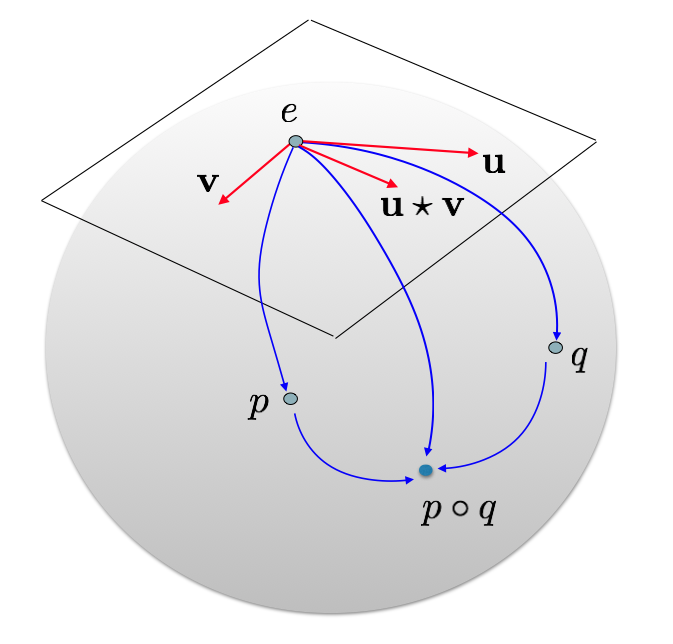
\includegraphics[scale=0.35]{figures/log_composition.png}
	\caption{graphical visualization of the Lie log-composition.}
	\label{fig:composition}
\end{figure}

\noindent
Following properties holds for the Lie log-composition:
\begin{enumerate}
	\item $\mathfrak{g} $ with the Lie log-composition $\oplus$ is a local topological non-commutative group (local group for short): if $C_{\mathfrak{g}}$ is the internal cut locus of $\mathfrak{g}$ then:
	\begin{enumerate}
		\item $(\mathbf{u}_{1}\oplus\mathbf{u}_{2}) \oplus \mathbf{u}_{3}
		= \mathbf{u}_{1}\oplus(\mathbf{u}_{2} \oplus \mathbf{u}_{3})$ for all $\mathbf{u}_{1}, \mathbf{u}_{2}, \mathbf{u}_{3}$ in $C_{\mathfrak{g}}$.
		\item $\mathbf{u}\oplus\mathbf{0}  = \mathbf{0}\oplus\mathbf{u} = \mathbf{u}$ for all $\mathbf{u}$ in $C_{\mathfrak{g}}$.
		\item $\mathbf{u}\oplus(-\mathbf{u} ) = \mathbf{0}$ for all $\mathbf{u}$ in $C_{\mathfrak{g}}$.
	\end{enumerate}
	\item For all $t,s$ real, such that $(t+s)\mathbf{u}$ is in $C_{\mathfrak{g}}$,
	\begin{align*}
	(t\mathbf{u})\oplus (s\mathbf{u}) = (t+s)\mathbf{u}
	\end{align*}
	And in particular, if the Lie algebra $\mathfrak{g}$ has dimension $1$ the local group structure is compatible with the additive group of the vector space $\mathfrak{g}$.
\end{enumerate}

\noindent
The algebraic structure $(\mathfrak{g} , \oplus)$ is called Lie log-group. Additional observations on this algebraic structure in the particular case of diffeomorphisms, are proposed in the next chapter.

To compute the log-composition there is the Backer-Campbell-Hausdorff formula, or BCH for short\footnote{
	Ironically the equality was proven by Dynkin in 1947 \cite{dynkin1947calculation}. A nice introduction for the particular case of matrices can be found in \cite{hall2015lie}. For the general case \cite{klarsfeld1989baker}, \cite{serre2009lie}, and for application to medical imaging \cite{vercauteren08}.
} 
that provides the exact solution to the Log-composition: 

\begin{align*}
BCH(\mathbf{u},\mathbf{v}) 
= 
\mathbf{u} + \mathbf{v} + \frac{1}{2}[\mathbf{u},\mathbf{v}] + \frac{1}{12}([\mathbf{u},[\mathbf{u},\mathbf{v}]]
+ [\mathbf{v},[\mathbf{v},\mathbf{u}]]) - \frac{1}{24}[\mathbf{v},[\mathbf{u},[\mathbf{u},\mathbf{v}]]] +... 
\end{align*}
This expansion provides the most immediate way to obtain a numerical computation of $\mathbf{u}\oplus \mathbf{v}$, truncating its terms.

%
%% % % % % % % % % % % % % % % % % % % % % % % % % % % % % % % % % % % % % %
%% % SECTION
%% % % % % % % % % % % % % % % % % % % % % % % % % % % % % % % % % % % % % % 
%\section{Affine Exponential, Affine logarithm and affine log-composition}\label{se:affine_exp_log_comp}
%


% % % % % % % % % % % % % % % % % % % % % % % % % % % % % % % % % % % % % %
% % SECTION
% % % % % % % % % % % % % % % % % % % % % % % % % % % % % % % % % % % % % % 
\section{Affine Exponential, Affine Logarithm and Parallel Transport: Definition and Properties}\label{se:parallel_transport}

Considering a Lie Group $\mathbb{G}$ with a connection $\nabla$ (that provides geodesics and curvature over manifold on which no Riemannian metric has been defined, see \cite{do1992riemannian}), the vector field $\nabla_{U}(V)$ associates at each point of the manifold the projection on the tangent plane of the derivative of $U$ in the direction of $V$. 

One of the considerable consequences of the definition of the connection is the possibility of defining \emph{geodesics} between points $p$ and $q$ of the manifold without any Riemannian metric. If a Riemannian metric is also defined on the manifold $\mathbb{G} $ considered with a connection, then geodesics defined by the metric coincides with the geodesics defined by the connection only for the particular Levi-Civita connection (see \cite{do1992riemannian}). A curve $\gamma:[0,1]\rightarrow \mathbb{G}$ such that $\gamma(0)=p$ and $\gamma(1) = q$ is a \emph{geodesic} defined by the connection $\nabla$ if 
\begin{align}\label{def:geodesics_eq}
\nabla_{\dot{\gamma}}\dot{\gamma} = 0 %\qquad \qquad \forall t\in [0,1] 
\end{align}
This definition allows a new kind of exponential from the Lie algebra to the Lie group. Given the point $p$ and the tangent vector at this point $\mathbf{v} \in T_{p}\mathbb{G}\simeq \mathfrak{g}$ we define: 
\begin{align*}
\exp :  \mathbb{G}  \times \mathfrak{g}     &\longrightarrow \mathbb{G}  
\\ 
(p,\mathbf{v}) &\longmapsto \exp_{p}(\mathbf{v})  = \gamma(1; p,\mathbf{v})
\end{align*}
such that the curve $\gamma(t;p,\mathbf{v}) = \gamma(t)$ on $\mathbb{G}$ is the unique geodesic that satisfies $\gamma(0) = p$ and $\dot{\gamma}(0) =  \mathbf{v} $.
This second kind of exponential, that differs from the previous one by the fact that the tangent space that defines the Lie algebra is considered at the generic point $p$ of the Lie group, is called here \emph{affine exponential}.

\noindent
The inverse of the affine exponential, the \emph{affine logarithm} is defined as:
\begin{align*}
\log :  \mathbb{G}  \times \mathbb{G}   \longrightarrow T_{p}\mathbb{G}   \simeq \mathfrak{g} 
\\ 
(p,q) \longmapsto \log_{p}(q)  = \mathbf{v} 
\end{align*}
Where $\mathbf{v} $ is the tangent vector in $p$ at the geodesic $\gamma$ on $\mathbb{G} $ that satisfies $\gamma(0) = p$ and $\gamma(1) = q$.

For further details and properties we refer to the literature; in this introduction we wish to provide only the intuitive idea that it is possible to move on the fiber bundle of the Lie group, transporting in some sense a tangent vector defined at the identity on another tangent space. Certainly the Lie group possesses a unique Lie algebra, as the tangent space at some point (the group's identity by convention), but two different tangent space (so two times the same isomorphic Lie algebra structure) may not have the basis vectors oriented in the same direction. 

In this section we also introduce the concept of parallel transport for the Lie group $\mathbb{G}$. On this definition, again borrowed from differential geometry\footnote{
	For introduction and general definition: \cite{misner1973gravitation}, \cite{knebelman1951spaces}, \cite{kheyfets2000schild} and in particular 	\cite{warner} for a definition of tangent vector field well suited for the parallel transport. For medical imaging applications \cite{lorenzi2011schild}, \cite{pennec2011parallel}, \cite{lorenzi2013geodesics}, \cite{lorenzi2014efficient}.
}, relies a method for the computation of the log-composition developed in this research for the first time.

\begin{definition}
	Let $\mathbb{G}$ be a finite dimensional connected Lie group defined with a connection $\nabla$ and $V$ a $\mathcal{C}^{\infty}$ vector field defined over $\mathbb{G}$. Given $p,q \in \mathbb{G}$ and $\gamma : [0,1] \rightarrow \mathbb{G}$ such that $\gamma(0) = p$ and $\gamma(1) = q$, the vector $V_{p} \in T_{p}\mathbb{G}$, is \emph{parallel transported along $\gamma$} up to $T_{q}\mathbb{G}$ if $V$ satisfies
	\begin{align*}
	\forall t \in  [0,1]
	\qquad
	\nabla_{\dot{\gamma}}V_{\gamma(t)} = 0
	\end{align*}
	The \emph{parallel transport} is the function that maps $V_{p}$ from $T_{p}\mathbb{G}$ to $T_{q}\mathbb{G}$ along $\gamma$:
	\begin{align*}
	\Pi(\gamma)_{p}^{q} :  T_{p}\mathbb{G} & \longrightarrow T_{q}\mathbb{G}  \\
	V_{p}&\longmapsto \Pi(\gamma)_{p}^{q}(V_{p}) = V_{q}
	\end{align*}
\end{definition}
\noindent
In the next properties we explore how did parallel transport and affine exponential behave when expressed as a composition and when the signs change.
\begin{prop}[Inversion]
	$\mathbb{G}$ Lie group, $\nabla$ connection, $p,q\in\mathbb{G}$. Given $\gamma$ such that $\gamma(0)= p$, $\gamma(1)=q$ and $\mathbf{u}\in T_{p}\mathbb{G}$, we have:
	\begin{enumerate}
	\item $\Pi(\gamma)_{p}^{q}(-\mathbf{u}) = -\Pi(\gamma)_{p}^{q}(\mathbf{u}) )$
	\item $q = \exp_{p}(\mathbf{u}) \phantom{z} \Longleftrightarrow \phantom{z} p = \exp_{q}(-\Pi(\gamma)_{p}^{q}(\mathbf{u}))$
	\end{enumerate}
\end{prop}

\begin{figure}[htbp]
	\centering
	\begin{minipage}[b]{3cm}
		\hspace{-4cm}
		\centering
		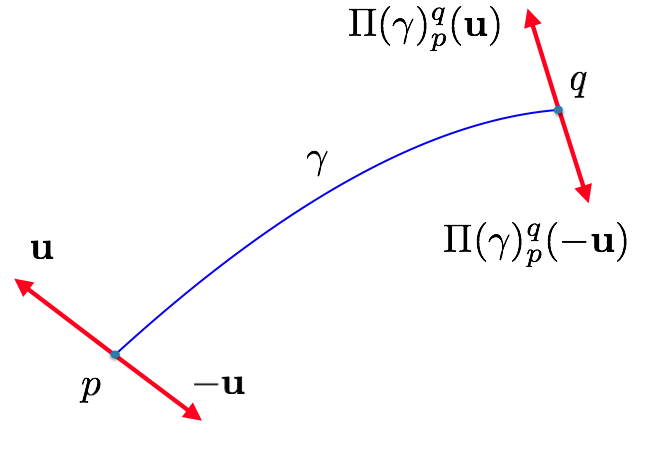
\includegraphics[width=6.5cm]{figures/inversion_1.png}
		\caption{First inversion property.}
		\label{fig:inversion_propr1}
	\end{minipage}
	\ \hspace{9mm} \
	\begin{minipage}[b]{4cm}
		\centering
		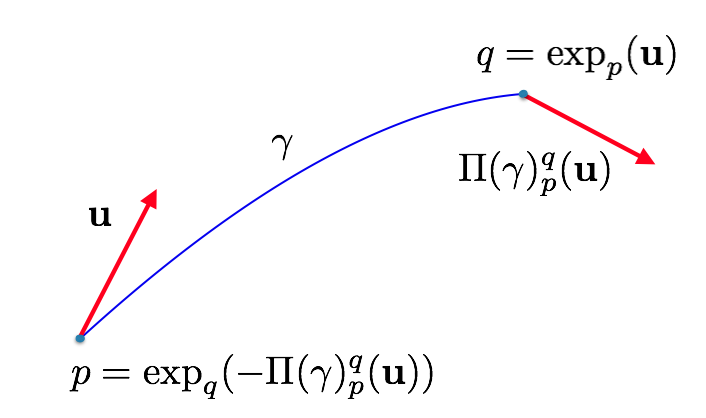
\includegraphics[width=6.5cm]{figures/inversion_2.png}
		\caption{Second inversion property.}
		\label{fig:inversion_propr2}
	\end{minipage}
\end{figure}
\begin{prop}[change of signs of the composition for affine exponential]
	$\mathbb{G}$ Lie group, $\nabla$ connection, $p,q\in\mathbb{G}$, $\mathbf{u}\in T_{p}\mathbb{G}$, $\mathbf{v}\in T_{q}\mathbb{G}$ and $q=\exp_{p}(\mathbf{u})$. Let $\beta$ be the tangent curve to $\mathbf{u}$ at $p$ such that $\beta(1) = q$ and $r= \exp_{b}(\mathbf{v})$. Given $\mathbf{w} \in T_{p}\mathbb{G}$ such that 
	\begin{align*}
	\exp_{p}(\mathbf{w}) = \exp_{q}(\mathbf{v}) \circ \exp_{p}(\mathbf{u})
	\end{align*}
	Then
	\begin{align*}
	\exp_{p}(-\mathbf{w}) = \exp_{\beta(-1)}(-\Pi(\beta)_{q}^{\beta(-1)}(\mathbf{v})) \circ \exp_{p}(-\mathbf{u})
	\end{align*}
\end{prop}

\begin{figure}[htbp]
	\centering
	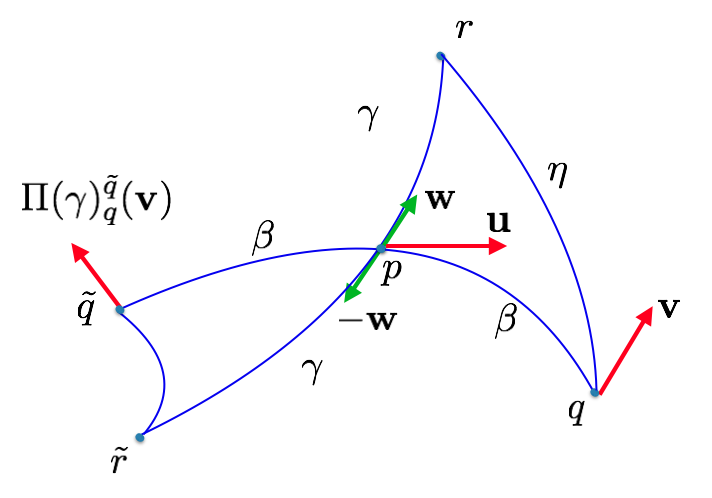
\includegraphics[width=9.5cm]{figures/sign_1.png}
	\caption{Change of sign property.}
	\label{fig:sign_propr}
\end{figure}

\begin{lemma}
	Let $\mathbb{G}$ be a finite dimensional connected Lie group defined with a Cartan connection $\nabla$ and $\mathbf{u}$ tangent vector in $ T_{e}\mathbb{G}$. Let $\gamma$ be a geodesic defined on $\mathbb{G}$ such that $\gamma(0) = e$, $\dot{\gamma}(0) =\mathbf{u}$ and $p = \gamma(1)$, point in the Lie group. Let $\beta$ be the curve over $\mathbb{G}$ defined as $\beta(t) = p\circ \gamma(t)$, then the two following conditions hold:
	\begin{enumerate}
		\item If $\nabla$ is a Cartan connection then $\beta$ is a geodesic.
		\item For $\mathbf{u}_{p} := D(L_{p})_{e}(\mathbf{u}) \in T_{p}\mathbb{G}$, push forward of the left-translation:
		\begin{align}\label{eq:lemma_pt}
		\exp_{p}(t\mathbf{u}_{p}) = p\circ \exp_{e}( t D(L_{p^{-1}})_{p}(\mathbf{u}_{p}) ) 
		= p\circ \exp_{e}(t\mathbf{u})
		\end{align}
	\end{enumerate}
\end{lemma}

\noindent
The following theorem is an application of the pole ladder \cite{lorenzi2011schild} for the computation of the exponential that will underpin one of the numerical methods for the computation of the log-composition. The main construction involved can be visualized in figure \ref{fig:theorem_pict}.
\begin{theorem}\label{th:local_approximation_theorem}
	Let $\mathbb{G}$ be a finite dimensional connected Lie group defined with a Cartan connection $\nabla$. 
	If, for each couple of linearly independent vectors $\mathbf{u}, \mathbf{v} \in T_{e}\mathbb{G}$, the following conditions hold:
	\begin{align*}
	a = \exp_{e}(\mathbf{u}) 
	\quad & \quad  
	b = \exp_{e}(\mathbf{v}) \\
	\mathbf{v}_{a}^{\parallel} = & \Pi(\gamma)_{e}^{a}(\mathbf{v})\\
	\gamma : [0,1] \rightarrow \mathbb{G} &\quad \gamma(0) = e \quad \dot{\gamma}(0) = \mathbf{u}
	\end{align*}
	\begin{align*}
	 \mathbf{v}^{\parallel} := D(L_{a^{-1}})_{e}( -\Pi(\alpha)_{a}^{e}(\mathbf{v}_{a}^{\parallel}))
	\end{align*}
	Then it follows that if $\mathbf{u}$ is in the open ball $B(\mathbf{0}, \epsilon)$, then exists a  $\tilde{\epsilon}>0$ such that $\mathbf{u}_{e}^{\parallel}$ belongs to $B(\mathbf{0}, \tilde{\epsilon})$, and exists a $\delta(\epsilon + \tilde{\epsilon})>0$ such that the inequality
	\begin{align*}
		\euclideanMetric{
			\log(\exp_{e}(\mathbf{v}^{\parallel} ))
			-
			\log(\exp_{e}\big(\frac{\mathbf{u}}{2}\big)   
				\circ  \exp_{e}(\mathbf{v}) 
				\circ \exp_{e}\big(-\frac{\mathbf{u}}{2}\big))
			} <\delta(\epsilon + \tilde{\epsilon})
	\end{align*}
	holds.
\end{theorem}
\noindent
The last statement can be rewritten as the approximation:
\begin{align}\label{eq:parallel_transport_main_approximation}
\exp_{e}(\mathbf{v}^{\parallel}) 
\simeq
\exp_{e}\big(\frac{\mathbf{u}}{2}\big)   
\circ  \exp_{e}(\mathbf{v}) 
\circ \exp_{e}\big(-\frac{\mathbf{u}}{2}\big)
\end{align}
that will turn out to be the main tool for the computation of the log-composition using parallel transport.\\
\begin{figure}[htbp]
	\centering
	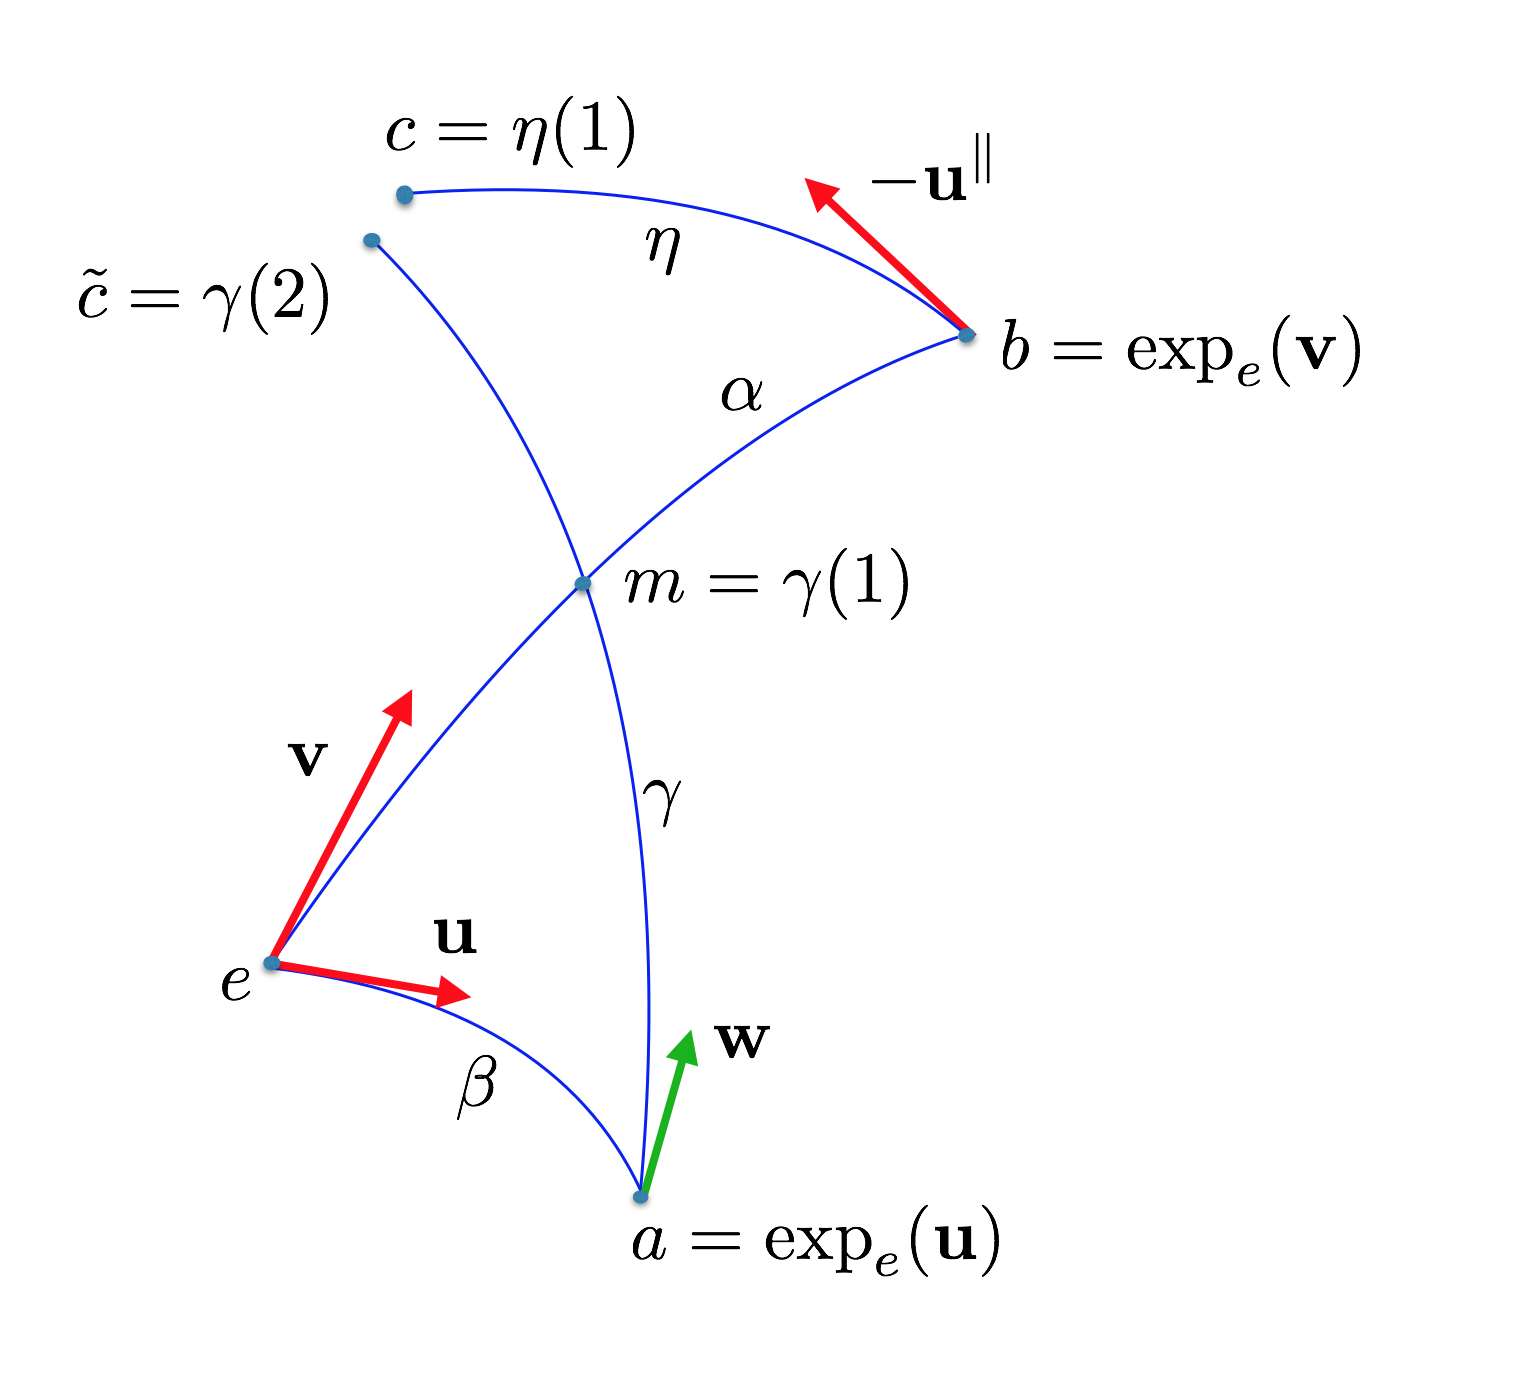
\includegraphics[width=9.5cm]{figures/theorem_pict.png}
	\caption{Pole ladder applied to parallel transport.}
	\label{fig:theorem_pict}
\end{figure}

When considering the equation \ref{eq:lemma_pt}, we use implicitly the formula for the change of base for affine exponential and logarithm \cite{arsigny2006bi}. It is in fact possible, using the derivative of the left-translation $L_{p}$, to bring back the $\exp$ and the $\log$ functions based at the point $p$ of the manifold to the $\exp$ and the $\log$ evaluated at the identity using the following formulas:
\begin{align}\label{eq:DL_DR}
\log _{p}(q)  &= DL_{p}(e) \log _{e}(q)  \\
\exp _{p}(\mathbf{u})  &= p\circ \exp_{e} (DL_{p}(e)^{-1} \mathbf{u})
\end{align}
\noindent
Further theoretical developments are beyond the aim of this research, but the reader can refer to the bibliography.
In the next section we present the numerical methods for the computation of the log composition.



% % % % % % % % % % % % % % % % % % % % % % % % % % % % % % % % % % % % % %
% % SECTION
% % % % % % % % % % % % % % % % % % % % % % % % % % % % % % % % % % % % % %
\section{Numerical Computations of the Log-composition}

In this section we provide explicit formulas for the computation of the log composition:
\begin{align}\label{eq:general_numerical_log_composition}
\mathbf{v}_{1}\oplus \mathbf{v}_{2} =  \log(\exp(\mathbf{v}_1)\circ \exp(\mathbf{v}_2))
\end{align}
using the tools introduced in the previous sections.

% % % % % % % % % % % % % % % % % % % % % % % % % % % % % % % % % % % % % %
% % SUBSECTION
% % % % % % % % % % % % % % % % % % % % % % % % % % % % % % % % % % % % % % 
\subsection{Truncated BCH formula for the Log-composition}\label{se:bch_formula}

As said in the end of section \ref{se:lie_exp_log_comp_bch} the Lie log-composition posses a closed form, the BCH formula, defined as the solution of the equation $\exp(\mathbf{w}) = \exp(\mathbf{u}) \circ \exp(\mathbf{v})$, for $\bf{u}$ and $\bf{v}$ in the Lie algebra $\mathfrak{g}$:
\begin{align}\label{eq:bch_definition}
	BCH(\mathbf{u},\mathbf{v}) 
	= 
	\mathbf{u} + \mathbf{v} + \frac{1}{2}[\mathbf{u},\mathbf{v}] + \frac{1}{12}([\mathbf{u},[\mathbf{u},\mathbf{v}]]
	+ [\mathbf{v},[\mathbf{v},\mathbf{u}]]) - \frac{1}{24}[\mathbf{v},[\mathbf{u},[\mathbf{u},\mathbf{v}]]] +... 
\end{align}
It consists of an infinite series of Lie bracket whose asymptotic behaviour cannot be predicted only from the coefficient of each nested Lie bracket term. In practical applications it can be computed using its \emph{approximation of degree} $k$, defined as the sum of the BCH terms having no more than $k$ nested Lie bracket. This convention is also coherent with the degree of the BCH expressed as polynomial formal series of adjoint operators (see next section \ref{se:taylor_expansion}):
\begin{align*}
BCH^{0}(\mathbf{u},\mathbf{v}) &= \mathbf{u} + \mathbf{v} \\
BCH^{1}(\mathbf{u},\mathbf{v}) &=  \mathbf{u} + \mathbf{v} + \frac{1}{2}[\mathbf{u},\mathbf{v}] \\
BCH^{2}(\mathbf{u},\mathbf{v}) &=  \mathbf{u} + \mathbf{v} + \frac{1}{2}[\mathbf{u},\mathbf{v}] + \frac{1}{12}([\mathbf{u},[\mathbf{u},\mathbf{v}]] + [\mathbf{v},[\mathbf{v},\mathbf{u}]]) \\
BCH^{3}(\mathbf{u},\mathbf{v}) &=  \mathbf{u} + \mathbf{v} + \frac{1}{2}[\mathbf{u},\mathbf{v}] + \frac{1}{12}([\mathbf{u},[\mathbf{u},\mathbf{v}]] + [\mathbf{v},[\mathbf{v},\mathbf{u}]])- \frac{1}{24}[\mathbf{v},[\mathbf{u},[\mathbf{u},\mathbf{v}]]] 
\end{align*}
In numerical computations Lie brackets can become extremely little. This means that we may be interested, in this particular case to compute only the first of the two new addend added between the first and the second degree of the BCH formula. For these situations we define a rational degree for the truncated BCH formula:
\begin{align*}
BCH^{3/2}(\mathbf{u},\mathbf{v}) &=  \mathbf{u} + \mathbf{v} + \frac{1}{2}[\mathbf{u},\mathbf{v}] + \frac{1}{12}[\mathbf{u},[\mathbf{u},\mathbf{v}]]
\end{align*}
These formulas can be considered as a first step toward the numerical approximations of the log-composition $\mathbf{u}\oplus \mathbf{v}$. They still have some limitations as the fact that they do not provide any information about the error carried by each term. Additional limitation can be found when applied to stationary velocity fields. This will be one of the topic of section \ref{se:log_composition_SVF}.


% % % % % % % % % % % % % % % % % % % % % % % % % % % % % % % % % % % % % %
% % SUBSECTION
% % % % % % % % % % % % % % % % % % % % % % % % % % % % % % % % % % % % % % 
\subsection{Taylor Expansion Method for the Log-composition}\label{se:taylor_expansion}

A more sophisticated numerical method to manage the nested Lie brackets for the computation of the log-composition is based on the Taylor expansion. \\
As shown in the appendix of \cite{klarsfeld1989baker} the terms of the BCH can be recollected using the Hausdorff method: each of the therms containing the n-th power of the vector $\mathbf{v}$ are collected together in the formal series $V^{n}$. Therefore
\begin{align*}
%\mathbf{u}\oplus \mathbf{v}  
BCH(\mathbf{u},\mathbf{v}) 
= 
\mathbf{u} + V^{1} \mathbf{v} + V^{2} \mathbf{v} + V^{3} \mathbf{v} + \cdots
\end{align*}
Given the adjoint map:
\begin{align*}
ad_{\mathbf{u}} : \mathfrak{g}  & \longrightarrow \mathfrak{g}  
\\
\mathbf{v} &\longmapsto ad_{\mathbf{u}}   \mathbf{v} :=  [\mathbf{u}, \mathbf{v}]
\end{align*}
and the multiple adjoint maps, defined as:
\begin{align*}
\text{ad}_{\mathbf{u}}^{n} \mathbf{v} 
&:= [  \underbrace{   \mathbf{u},[\mathbf{u},... [\mathbf{u}}_{\text{n-times}},\mathbf{v}]...]] 
\\
\\
\text{ad}_{\mathbf{u}}^{-n} \mathbf{v} 
&:= [[...[  \mathbf{v}, \underbrace{   \mathbf{u}]...],\mathbf{u}}_{\text{n-times}}]
= (-1)^n \text{ad}_{\mathbf{u}}^{n} \mathbf{v} 
\end{align*}
it can be proved that then the operator $V^{1}$ is applied to $\mathbf{v}$, it provides the linear part of $\mathbf{v}$ in the BCH formula. It results
\begin{align*}
V_{1}
= 
\frac{  
	\text{ad}_{\mathbf{u}}^{-1} 
	}{
	\exp{(\text{ad}_{\mathbf{u}})}-1
	}
=
\sum_{n=0}^{\infty} \frac{(-1)^nB_{n}}{n!} \text{ad}_{\mathbf{u}}^{ - n} 
=
\sum_{n=0}^{\infty} \frac{B_{n}}{n!} \text{ad}_{\mathbf{u}}^{ n} 
\end{align*}
where $\lbrace B_{n} \rbrace_{n=0}^{\infty} $ is the sequence of the second-kind Bernoulli number. If first-kind Bernoulli number are used, then each term of the summation must be multiplied for $(-1)^{n}$, as did for example in \cite{klarsfeld1989baker}. The denominator is defined within the structure of the formal power series ring \cite{mariconda2013calcolo}.\\
In conclusion, the log-composition can expressed as:
\begin{align*}
\mathbf{u}\oplus \mathbf{v}  
&= 
\mathbf{u} + 
\frac{  
	\text{ad}_{\mathbf{u}}^{-1} 
}{
\exp{(\text{ad}_{\mathbf{u}})}-1
} \mathbf{v}  
+ 
\mathcal{O}(\mathbf{v} ^2) 
\end{align*}
\begin{align}\label{eq:taylor}
\mathbf{u}\oplus \mathbf{v}  
&=
\mathbf{u} 
+
\sum_{n=0}^{\infty} \frac{B_{n}}{n!} \text{ad}_{\mathbf{u}}^{ n} 
\mathbf{v}  
+
\mathcal{O}(\mathbf{v} ^2)
\end{align}
that will turn out to be an important tool for the computation of the log-composition in the finite dimensional case. 

% % % % % % % % % % % % % % % % % % % % % % % % % % % % % % % % % % % % % %
% % SUBSECTION
% % % % % % % % % % % % % % % % % % % % % % % % % % % % % % % % % % % % % % 
\subsection{Parallel Transport Method for the Log-composition}
To obtain a numerical computation for the log-composition using parallel transport, we have to consider two assumptions: 
\begin{enumerate}
	\item If $\mathbf{v}^{\parallel} $ is defined as in theorem \ref{th:local_approximation_theorem}, then exists an $\hat{\epsilon} > 0$ such that
	\begin{align*}
	\euclideanMetric{
		\mathbf{u}\oplus \mathbf{v}  
		-
		(
		\mathbf{u} + \mathbf{v}^{\parallel} 
		)
	} <\hat{\epsilon}
	\end{align*}
	\item If the vector $\mathbf{w}\in\mathfrak{g}$ is small enough, then:
		\begin{align*}
		\exp(\mathbf{u}) \simeq e + \mathbf{u}
		\end{align*}
\end{enumerate}
The first assumption is a consequence of geometrical intuition, while
the second one is valid under the Lipschitz hypothesis stated in proposition 8.6 pag. 163 \cite{younes2010shapes} holds and a deepening in this beyond the aim of this research. For our purposes we will consider the vector $\mathbf{w}$ small enough to make the approximation questioned here reasonable.

From these assumptions and from equation \ref{eq:parallel_transport_main_approximation} it follows that 
\begin{align*}
\mathbf{u}\oplus \mathbf{v}
&\simeq
\mathbf{u} + \mathbf{v}^{\parallel}
\\
e + \mathbf{v}^{\parallel}
&\simeq
\exp_{e}\big(\frac{\mathbf{u}}{2}\big)   
\circ  \exp_{e}(\mathbf{v}) 
\circ \exp_{e}\big(-\frac{\mathbf{u}}{2}\big)
\end{align*}
Therefore
\begin{align}\label{eq:parallel_transport}
\mathbf{u}\oplus \mathbf{v}
&\simeq
\mathbf{u} 
+
\exp_{e}\big(\frac{\mathbf{u}}{2}\big)   
\circ  \exp_{e}(\mathbf{v}) 
\circ \exp_{e}\big(-\frac{\mathbf{u}}{2}\big)
 -
 e
\end{align}
With the truncated BCH and the Taylor expansion, this is the third numerical method for the computation of the log-composition explored in this thesis.\\
We have to notice that when we apply it on the infinite dimensional case, the approximation \ref{eq:parallel_transport} holds under the following additional assumption:
\begin{enumerate}
\item[3.] Theorem \ref{th:local_approximation_theorem} holds when the Lie group is infinite dimensional.
\end{enumerate}
An eventual confirmation is at the moment not known to the author. We assume it is true in coherence with what has been said in the introduction, section \ref{se:diffe_util_and_liab}.










